\documentclass[border=3pt]{standalone}
% Preâmbulo compartilhado pelos diagramas TikZ da aula 14 (SLAM com EIF)
\usepackage[T1]{fontenc}
\usepackage[utf8]{inputenc}
\usepackage{lmodern}
\usepackage{amsmath}
\usepackage{xcolor}
\usepackage{tikz}
\usetikzlibrary{arrows.meta,angles,quotes,decorations.pathmorphing,decorations.pathreplacing,calc,
                positioning,shapes.geometric,shapes.misc,backgrounds,fit,
                math}

% Paleta (mesma dos SVGs originais)
\definecolor{dblue}{HTML}{2A5B8C}
\definecolor{dorange}{HTML}{B3541E}
\definecolor{dgreen}{HTML}{4A7C59}
\definecolor{dred}{HTML}{9C4B4B}
\definecolor{dcream}{HTML}{F4F1EA}
\definecolor{dshade}{HTML}{DDD7C9}

% Função gaussiana (não normalizada por padrão de escala visual)
\pgfmathdeclarefunction{gauss}{3}{%
  \pgfmathparse{1/(#3*sqrt(2*pi))*exp(-((#1-#2)^2)/(2*#3^2))}%
}

% Estilos comuns (prefixo d... para não colidir com chaves internas do pgf)
\tikzset{
  >={Stealth[length=2mm]},
  dguide/.style={gray!55, dashed, line width=0.4pt},
  daxis/.style={gray!60, line width=0.7pt, ->},
  dbody/.style={fill=black!3, draw=black!80, line width=1pt},
  dacc/.style={draw=dblue, line width=1pt},
  dlbl/.style={black!55, font=\small},
  dsub/.style={black!45, font=\footnotesize},
  dstate/.style={circle, draw=black!80, fill=dcream, line width=1pt,
                 minimum size=17mm, font=\large, inner sep=1pt},
  dobs/.style={circle, draw=black!80, fill=dshade, line width=1pt,
               minimum size=14mm, font=\large, inner sep=1pt},
  dbox/.style={rounded corners=2pt, draw=black!80, fill=dcream, line width=1pt,
               align=center, inner sep=6pt},
  dop/.style={circle, draw=black!80, fill=white, line width=1pt,
              minimum size=6mm, inner sep=0pt, font=\small},
  dtrans/.style={->, dblue, line width=1pt},
  dmeas/.style={->, dorange, line width=1pt},
  dcurve/.style={line width=1pt, dblue},
  dcurveb/.style={line width=1.4pt, dorange},
}

\begin{document}
\hyphenpenalty=10000 \exhyphenpenalty=10000 \tolerance=9999 \emergencystretch=3em
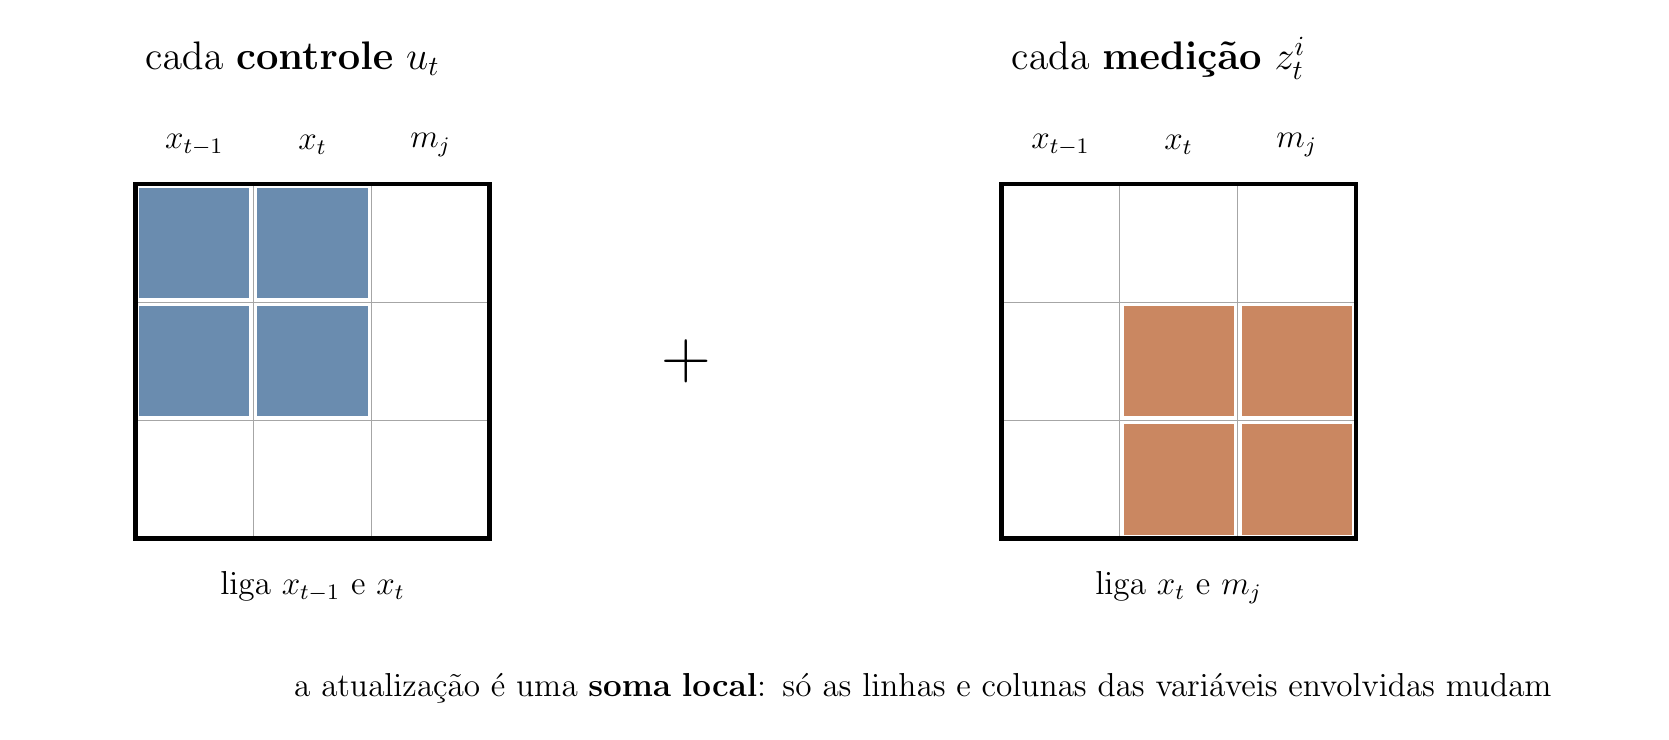
\begin{tikzpicture}[x=1cm,y=1cm]
\def\cw{1.5}
\tikzset{g/.style={draw=black!35, line width=0.5pt}}
\foreach \o/\tit/\a/\b/\col/\leg in {0/{cada \textbf{controle} $u_t$}/0/1/dblue/{liga $x_{t-1}$ e $x_t$}, 11/{cada \textbf{medição} $z_t^i$}/1/2/dorange/{liga $x_t$ e $m_j$}} {
  \node[font=\Large, anchor=west] at (\o,1.6) {\tit};
  \foreach \i in {0,1,2} {\foreach \j in {0,1,2} {\draw[g] ({\o+\j*\cw},{-\i*\cw}) rectangle ({\o+(\j+1)*\cw},{-(\i+1)*\cw});}}
  \foreach \p in {\a,\b} {\foreach \q in {\a,\b} {\fill[\col!70] ({\o+\q*\cw+0.05},{-\p*\cw-0.05}) rectangle ({\o+(\q+1)*\cw-0.05},{-(\p+1)*\cw+0.05});}}
  \draw[line width=1.6pt] (\o,0) rectangle ({\o+3*\cw},{-3*\cw});
  \node[font=\large] at ({\o+0.75},0.5) {$x_{t-1}$}; \node[font=\large] at ({\o+2.25},0.5) {$x_t$}; \node[font=\large] at ({\o+3.75},0.5) {$m_j$};
  \node[font=\large, anchor=north, text width=7cm, align=center] at ({\o+2.25},-4.8) {\leg};}
\node[font=\Large\bfseries] at (7.0,-2.25) {\Huge $+$};
\node[font=\large, text width=18cm, align=center] at (10.0,-6.4) {a atualização é uma \textbf{soma local}: só as linhas e colunas das variáveis envolvidas mudam};
\end{tikzpicture}
\end{document}
